\documentclass[12pt]{article}
\renewcommand{\familydefault}{\sfdefault}
\usepackage{csvsimple}
\usepackage{graphicx}
\usepackage{hyperref}
\parindent=0pt
\parskip=5 pt
\setlength{\textwidth=7in}
\setlength{\oddsidemargin=-.25 in}
\setlength{\topmargin=0 in}
\setlength{\textheight=8.5 in}
%\usepackage{draftwatermark}
%\SetWatermarkText{Draft}
%\SetWatermarkScale{5}
\title{DUNE Offline Computing Model Calculations for 2023 FCSRG}
\author{H. Schellman for the Computing Consortium}
\date{\today -- version 2}



\newcommand{\hrefII}[1]{\href{#1}{#1}}
\begin{document}


\makeatletter
\csvset{
  autotabularright/.style={
    file=#1,
    after head=\csv@pretable\begin{tabular}{|*{\csv@columncount}{r|}}\csv@tablehead,
    table head=\hline\csvlinetotablerow\\\hline,
    late after line=\\,
    table foot=\\\hline,
    late after last line=\csv@tablefoot\end{tabular}\csv@posttable,
    command=\csvlinetotablerow},
}
\makeatother
\newcommand{\csvautotabularright}[2][]{\csvloop{autotabularright={#2},#1}}

\maketitle

This is similar to the version shown to the CCB in December and listed in docdb 27462\cite{CCB2023Minutes}.  Change is raising of FNAL contribution from 25 to 40\% for disk and CPU.  

\section{Introduction}

This is an annual projection for DUNE CPU and storage needs intended for use at the Fermilab Computing Resource Scrutiny Meeting in February 2023\cite{FCRSG2023}.  It is based on the requests at the DUNE Computing Contributions Board meeting in December 2022 but with a different mix of resource requests from Fermilab to better match the pledges received at the CCB. 

The overall computing model  and 2022 projections for DUNE are described in chapters 6-13 of the recent (Oct. 2022) DUNE Conceptual Design Report \cite{DUNE:2022fcw}.   This document provides updates on resource needs for 2023. 

The 2023 projection is done using codes at: \href{https://github.com/DUNE/CCB-data/tree/master/Numbers-2023}{https://github.com/DUNE/CCB-data/tree/master/Numbers-2023} from parameters stored in a json file. We use CPU and storage sizes derived from protoDUNE and simulation experience and apply them to projected numbers of events from the various DUNE detectors. 

Details are provided in the appendices while the main body of this note summarizes pledges, usage and projected need for the CCB with revisions in February 2023. 




Changes since the last report include:

\begin{itemize}
\item A later start for ProtoDUNE-2 running at CERN. This leads to a spike in needs for storage/CPU needs in late CY2023. 
\item Use of memory-weighted-core time instead of wall-time as our codes often require more memory than is available on a single core.  This means that our jobs sometimes need to reserve more than one core for a single process. This motivates the introduction of a memory-weighted wall-time unit for contributions  as different sites will  need to provide different amounts of wall-time to perform the same processing. 
\item Revisions to near-term requests based on the 2022 experience including a hold on tape requests from the collaboration during protoDUNE activities. 
\item Simulation disk copies has been reduced from 2 to 1.5 to fit within a reasonable profile.  If more disk becomes available we can restore more simulation copies.  
\item A change in future tape requests to reflect the greater accessibility of tape archives at CERN and FNAL relative to other sites. 
\end{itemize}

Proposed pledges for 2023 are detailed  in sections: Disk(\ref{sec:diskresult}), Tape(\ref{sec:taperesult}) and CPU(\ref{sec:cpuresult} )below.   %A summary of requests for 2023 is shown here in Table \ref{tab:summary2023}.

%\begin{table}[ht]
%\begin{centering}
%
%\begin{tabular}{|ll|rr|r|r|}
%\hline
% 	&&	Disk (PB)	&	Modified Disk (PB)	&	Tape(PB)	&	CPU (MWC-years)	\\
%	\hline
%{\bf Model}	&&	25.80	&	25.80	&	45.5	&	15,169	\\
%\hline
%{\bf Request}	&&		&		&		&		\\
%&FNAL	&	7.80	&	8.86	&	36.2	&	3,792	\\
%&CERN	&	2.60	&	4.00	&	9.2	&	3,792	\\
%&National	&	15.40	&	12.94	&	0.1	&	7,585\\
%\hline
%&{\bf Total}	&	25.80	&	25.80	&	45.5	&	15,169	\\
%\hline
%\end{tabular}
%
%\caption{Proposed pledges for 2023.  Disk pledges are based on existing CERN and FNAL contributions with National contributions making up the rest of the model request.  Tape pledges reflect the dominant use of CERN and FNAL for archival storage of data.  CPU pledges are in units of memory-weighted-core-years and assume Fermilab and CERN each pledge 25\%.   }
%\end{centering}
%\label{tab:summary2023}
%\end{table}


\clearpage

\section{Disk and Tape}

Generally, raw data are stored on tape at both CERN and FNAL.  Simulation and reconstructed data  have one tape copy at Fermilab and recent reconstructed and simulated samples have one (or two) disk copies with one at Fermilab and one in Europe.  Appendix \ref{storage} gives details on the size and types of data from the SAM data catalog.

CERN and FNAL have special responsibilities for archival data storage and for disk space for raw data while contributions from  other collaborating institutions are aggregated under the heading National, which includes US sites outside of FNAL.  A revised split between FNAL, CERN and National contributions until 2027 is shown in Table \ref{tab:division}.  The pledges proposed to the 2023 CCB deviated slightly from those numbers with larger contributions from the host laboratories in 2023 due to resources already in place.  In the later part of this document we have adjusted the split to reflect the reality of the FNAL/CERN/National split more closely. 

\begin{table}[h]
\begin{centering}
%\caption{Division between FNAL/CERN/National for storage until 2027}
%{\bf Tape}
%\begin{tabular}{|rrrr|}
%\hline
% &FNAL&CERN & National \\
% \hline
%Raw:&  0.5&  0.5&  0.0\\
%Sim:& 1.0&   0.0&   0.0\\ 
%Reco-Data:& 1.0&   0.0&   0.0\\
%Test: &  0.5&   0.5&  0.0\\
%
% \hline
%  \end{tabular}

   {\bf Disk}
     \begin{tabular}{|rrrr|}
     \hline
 &FNAL&CERN & National \\
 \hline
 Raw&   0.50&   0.50&  0.00\\ 
 Sim: & 0.40&  0.1&  0.50\\
  Reco-Data: &  0.4&   0.10&  0.50\\ 
  Test: &  0.50& 0.50&   0.00\\
  \hline
   \end{tabular}
  \caption{Proposed division between FNAL/CERN/National for storage until 2027.   The tape division is not yet finalized as we work on integration of National tape archives. In the long run, National sites are expected to take over from CERN. The FNAL/CERN/other split for disk has changed. }

   \label{tab:division}
   \end{centering}
   \end{table}

\subsection{Disk}
Table \ref{tab:RSEUsage} summarizes the disk utilization known to rucio, augmented with information gathered from individual sites at a meeting on 2022-11-21.  Some sites, notably TIFR, are not yet fully integrated so do not show up in the rucio reports, while others (PIC) are still being filled.  The contributions listed in Table \ref{tab:DiskPledges} sum the rucio and non-rucio disk known to be allocated to DUNE.

Figure \ref{fig:Cumulative-Disk}  summarize the cumulative disk needs and requests projected by our model. These numbers are used to generate the request for 2023.  They are divided into the two host laboratories (CERN and FNAL) and National, which includes contributions from the rest of the collaboration, including OSG, BNL and NERSC in the US. 

Table \ref{tab:DiskPledges} summarizes the pledges from previous years compared to the actual amounts allocated and used from Table \ref{tab:RSEUsage} .   The 2023 request has been re-evaluated in light of underuse in 2021 and 2022 and should better match the likely capacity of the collaborating sites.  It is however, still higher than 2022 due to ProtoDUNE running and increased simulation for the far and near detectors. 

%\begin{table}[ht]
%\centering\csvautotabularright{external/DUNERSEUSAGE-2022-11-14.csv}
%\caption{Summary  of DUNE disk areas known to rucio \cite{scotgrid}.  The CASTOR and FNAL Dcache areas are partially tape-backed and expandable. FNAL and CERN allocations are not provided by the reports but usage is.  }
%\label{tab:RSEUsage}
%\end{table}
\begin{table}[ht]
\centering\csvautotabularright{external/DiskSummary-2022-11-28.csv}
\caption{Disk allocations and usage across sites.    These numbers are derived from rucio reports and from cross-checks with individual sites on 2022-11-21. }
\label{tab:RSEUsage}
\end{table}

\begin{figure}[h]
\centering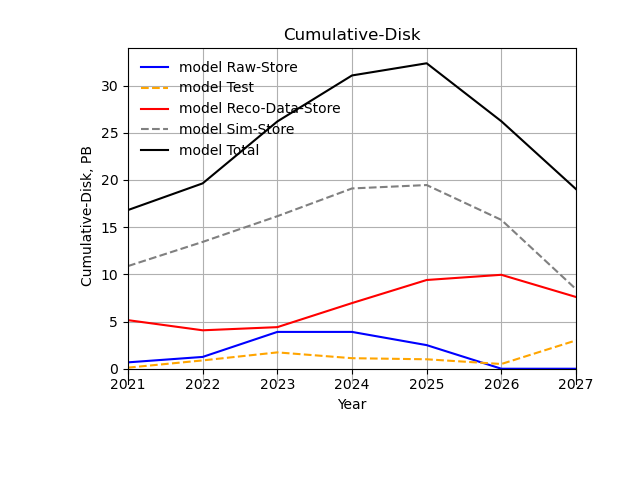
\includegraphics[height=0.5\textwidth]{MoreSim_2023-01-31-2027/MoreSim_2023-01-31-2027-Cumulative-Disk.png}
\csvautotabularright{MoreSim_2023-01-31-2027/MoreSim_2023-01-31-2027-Cumulative-Disk-Source.csv}
\csvautotabularright{MoreSim_2023-01-31-2027/MoreSim_2023-01-31-2027-Cumulative-Disk-Request.csv}
\caption{Cumulative Disk needs in PB. Includes data lifetimes.  The top table shows the source of the data while the bottom table  shows the proposed split using the fractions from Table \ref{tab:division}.  }\label{fig:Cumulative-Disk}
\end{figure}




\begin{table}[ht]
\centering\csvautotabularright{external/DiskResources-2021-2022-2023-Detail-pledged.csv}
\caption{Summary of disk pledges, allocations and usage for 2021-2022 with model request and pledges 2023 .  The NL is assumed to stay constant as no new pledge was recorded. This is based on the 2022/2023 CCB tables which are available in indico  \cite{CCB2022,CCB2023}.  The usage numbers are derived from the rucio reports in Table \ref{tab:RSEUsage} and may not be complete.  }
\label{tab:DiskPledges}
\end{table}

\subsubsection{Conclusion}\label{sec:diskresult}
The overall request for 2023 is 25.8 PB vs. the 22.6 PB already on the floor so we need to find 3.2 PB or descope the number of copies on disk. Currently CERN and FNAL contribute more  (12.9 PB on the floor vs. 9.1 PB request) than they would under the current divisions in Table \ref{tab:division} while national contributions are currently 9.7 PB vs 15.4 in the request based on the allocations in Table \ref{tab:division}.   We have readjusted the proposed contributions to better reflect the CERN/FNAL contributions. 


\clearpage
\subsection{Tape}



Figure  \ref{fig:Cumulative-Tape}  summarizes the cumulative  tape need projected by our model. These numbers are used to generate the requests for 2023.  They are divided into the two host laboratories (CERN and FNAL) and National, which includes contributions from the rest of the collaboration, including OSG, BNL and NERSC in the US. 


\subsubsection{Conclusion}\label{sec:taperesult}
DUNE currently has $\sim$23 PB of data on tape at Fermilab and 5 PB of protoDUNE data as a second copy at CERN.  We anticipate needing up to 45 PB of tape (an increase of 16 PB from 2022) to accommodate the ProtoDUNE run 2 data and increased simulation. 

The UK and the IN2P3 have made $\sim 3$ PB of tape archive available but it has not yet been smoothly integrated into our data flow.  We  therefore substantially reduce our request for these resources to $\sim 100$ TB per site, to allow testing of integration, with an increased request anticipated future years. 

\begin{figure}[h]
\centering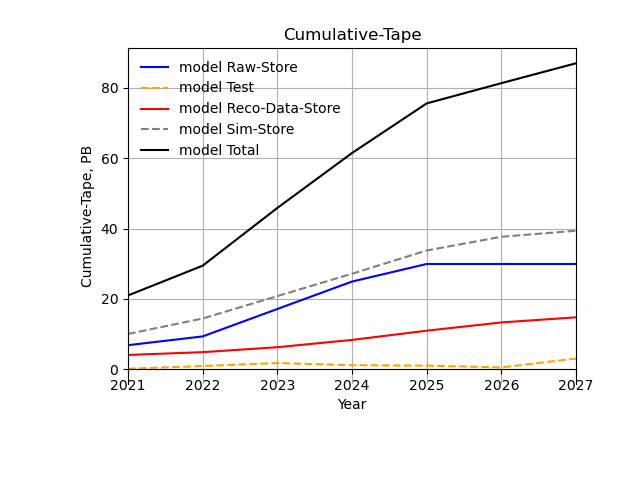
\includegraphics[height=0.4\textwidth]{MoreSim_2023-01-31-2027/MoreSim_2023-01-31-2027-Cumulative-Tape.png}

\csvautotabularright{MoreSim_2023-01-31-2027/MoreSim_2023-01-31-2027-Cumulative-Tape-Source.csv}
%\csvautotabularright{external/MoreSim_2022-12-02-2026-Cumulative-Tape-Request.csv}
\csvautotabularright{MoreSim_2023-01-31-2027/MoreSim_2023-01-31-2027-Cumulative-Tape-Request.csv}
\caption{Cumulative Tape requests in PB, includes data lifetimes.  The top table shows the source of the data while the bottom table  shows the proposed split.  National contributions are set low in 2023 and grow thereafter as more tape archives are integrated. }\label{fig:Cumulative-Tape}
\end{figure}



\clearpage
\section{CPU Needs}

%Table \ref{tab:CPUUsage} shows pledges and utilization for 2021-2022 and the request for 2023.  

DUNE differs from other HEP experiments in frequently requiring more memory/core than is available at particular sites.  For example an 8-slot pilot with 16 GB of available memory may only accommodate four reconstruction processes.   As a result, we make our requests in terms of memory-weighted-core wall time (MWC)  with the base memory being 2000 MB. This maps reasonably well to the memory weighted slot-time returned by HTCondor and the slot-time reported in EGI statistics.  Sites that offer more  (or less) than 2000 MB/core can scale their contributions up by the local memory/core.

\subsection{Model calculation}
The wall-time estimates in the model are created by estimating the number of simulated and raw events taken and then scaling by the measured CPU time on a gpvm corrected to wall-time by the estimated efficiency (default 70\%) and for a memory utilization factor that takes into account the differing memory needs for different applications. Here we assume that analysis takes 3000 MB, reconstruction takes 4000MB, and simulation takes 6000MB.  Contributions are then requested in units of MWC-time which is wall-time$\times$2000 MB units. 


\begin{figure}[h]
\centering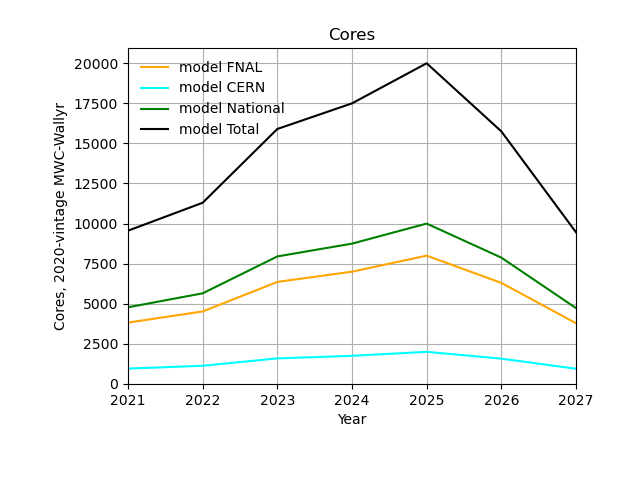
\includegraphics[height=0.4\textwidth]{MoreSim_2023-01-31-2027/MoreSim_2023-01-31-2027-Cores.png}
\csvautotabularright{MoreSim_2023-01-31-2027//MoreSim_2023-01-31-2027-Cores.csv}  %had to fix so moved to external
\caption{Proposed memory-weighted wall-time needs in number of 2000 MB cores (MWC-years). Memory-weighted  wall-time takes into account memory and efficiency.}\label{fig:CoresMain}
\end{figure}

Figure/Table \ref{fig:CoresMain} shows the projected memory-weighted wall-time  (MWChr) need projections through 2027.  This is different than in previous years where memory weighting was not applied.   They are divided into the two host laboratories (CERN and FNAL) and National, which includes contributions from the rest of the collaboration, including OSG, BNL and NERSC in the US. 


\subsection{Example of memory weighted pledges}
An example of a  national pledge in MWC might be  1000 cores with 2GB available/core, 500 cores with 4 GB available/core and 100 cores with 8 GB available/core.  The MWC pledge would then be 

\newcommand{\GB}{\hbox{GB}}

\begin{eqnarray*} 1000\times2\GB/2\GB &+& \\ 500\times4\GB/2\GB &+&\\100\times8\GB/2\GB\\&&= 2400 \hbox{\ MWC units}\end{eqnarray*}.

A pledge with cores with $<$ 2 GB would get partial MWC units per core. 

The idea here is make the additional load of running large DUNE jobs transparent to sites, which either need to provide more than 2GB of memory/job or assign more cores than are actually used to a given job.  How a site makes and meets a pledge is up to the site management. Table \ref{tab:VOcard} summarizes the memory specifications from existing "VO" cards for the different experiments.  DUNE and LHCb currently are the only ones with a stated maximum $>$ 2048 MB.

\subsection{Requests}




Table \ref{tab:CPUUsage} summarizes previous pledges\cite{CCB2022} and the measured usage  for 2021 and 2022 using FNAL's  HTCondor memory-weighted wall-time statistics\cite{fifemonDUNE}.  The  usage numbers for 2022 are Nov 2021 to Oct 2022. 

Table \ref{tab:EIGSummary} summarizes the statistics for European sites from Nov 2021 to Oct 2022 derived from the EGI accounting\cite{EGI2022} which uses the number of cores allocated to a pilot.   If four 4000 MB reconstruction jobs were sent to an 8-core pilot on a system with 2000MB/core, this would be equivalent to using 8 MWC (memory-weighted wall-time units).   This is therefore  more similar to the US MWC concept than to counting cores without reference to memory usage. 


\begin{table}[ht]
\centering\csvautotabularright{external/CPUresources-2021-2022-2023-v4.csv}
\caption{Summary  of DUNE wall-time pledges and contributions for 2021, 2022 and 2023.  The 2022 and 2023 actual  are memory-weighted core-years.  Individual nations are listed and then merged (with US OSG) into a National section.  Some international contributions (notably UK, NL and IN) come with very substantial memory per core and thus receive a large weighting in the MWC metric. The NL contribution has a * as we did not receive a formal pledge.} 
\label{tab:CPUUsage}
\end{table}

\begin{table}[ht]
\centering\csvautotabularright{external/EIG-2022.csv}
\centering\csvautotabularright{external/EIG-2022-National.csv}
\caption{Summary  of DUNE slot-years used for European collaborators, Nov. 21 to Oct. 22, using the EGI accounting\cite{EGI2022}.  The top shows all sites with EGI records, the bottom shows the summed contributions. These numbers reflect multiple-core slot reservations to account for larger memory use and are similar to, but  generally higher than, the FNAL accounting numbers in the previous table.} \label{tab:EIGSummary}
\end{table}

\begin{table}[ht]
\centering
\begin{tabular}{|l|l|l|}
\hline
Expt.&Max Memory& EGI VO Card\\
\hline
DUNE & 4000& \hrefII https://operations-portal.egi.eu/vo/view/voname/DUNE \\
ATLAS & 2000& \hrefII https://operations-portal.egi.eu/vo/view/voname/atlas \\
CMS & 2000& \hrefII https://operations-portal.egi.eu/vo/view/voname/cms \\
LHCb & 4000& \hrefII https://operations-portal.egi.eu/vo/view/voname/lhcb \\
ALICE& 2000& \hrefII https://operations-portal.egi.eu/vo/view/voname/alice \\
BelleII&2048& \hrefII https://operations-portal.egi.eu/vo/view/voname/belle \\
\hline
\end{tabular}
\caption{Maximum memory statements from the VO cards of major experiments.}
\label{tab:VOcard}
\end{table}

\pagebreak
\subsection{Conclusion}\label{sec:cpuresult} The advent of ProtoDUNE-2 running in 2023 and ramp-up of simulation for the FD and ND will lead to somewhat increased needs for CPU resources.  For 2023, we are requesting $\sim$12,800 memory-weighted core-years (MWC-years) where a system with 2000 MB/core is assumed to offer 1 MWC/core.  

%\section{
%\section{Projected Disk and Tape needs by source and site}
\begin{figure}[h]
\centering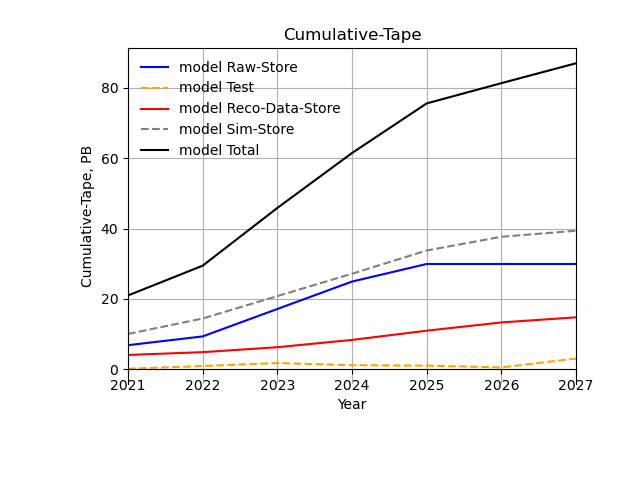
\includegraphics[height=0.4\textwidth]{MoreSim_2023-01-31-2027/MoreSim_2023-01-31-2027-Cumulative-Tape.png}
\csvautotabularright{MoreSim_2023-01-31-2027/MoreSim_2023-01-31-2027-Cumulative-Tape.csv}\caption{Cumulative Tape needs in PB. Includes multiple copies and data lifetimes. The top 4 lines show the source of the data while the last four propose responsibilities.}
\label{fig:Cumulative-Tape}
\end{figure}
\begin{figure}[h]
\centering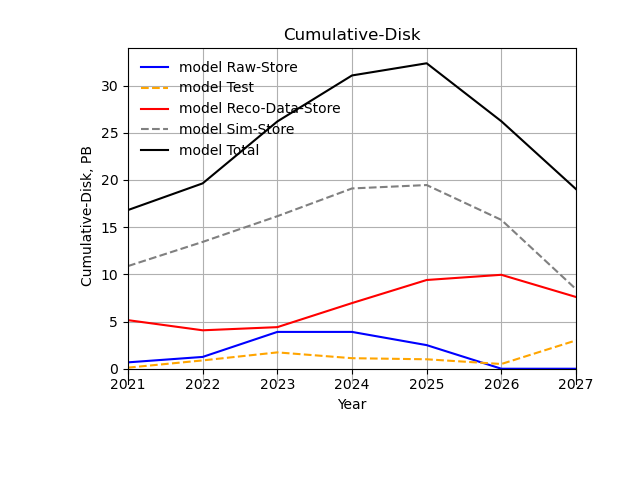
\includegraphics[height=0.4\textwidth]{MoreSim_2023-01-31-2027/MoreSim_2023-01-31-2027-Cumulative-Disk.png}
\csvautotabularright{MoreSim_2023-01-31-2027/MoreSim_2023-01-31-2027-Cumulative-Disk.csv}\caption{Cumulative Disk needs in PB. Includes multiple copies and data lifetimes. The top 4 lines show the source of the data while the last four propose responsibilities.}
\label{fig:Cumulative-Disk}
\end{figure}


%\section{Model Assumptions}

\cleardoublepage
%\renewcommand{\bibname}{References}
\bibliographystyle{utphys} 
\bibliography{bib}
\clearpage
\appendix

\section{Information about storage from SAM}\label{storage}

This section provides information on the sizes of data samples known to the SAM data catalog as of Nov. 1, 2022.  If a file has multiple copies, that is not shown here.  Tables \ref{tab:MCinSAM} and \ref{tab:DataInSam} show the total across all streams and data tiers while table \ref{tab:LargestSizes} shows the distribution of the largest samples.  


\begin{table}[ht]
 \centering\csvautotabularright{external/mc.csv}
\caption{Summary  of total simulation in SAM by detector type as of Nov 1, 2022.} 
\label{tab:MCinSAM}
\end{table}

\begin{table}[ht]
 \centering\csvautotabularright{external/detector.csv}
 \caption{Summary  of total detector data in SAM by detector type as of Nov 1, 2022.}
 \label{tab:DataInSam}
\end{table}



\begin{table}[ht]
 \centering\csvautotabularright{external/TOPTYPES.csv}
\caption{Classification of the largest data samples in SAM.  They are classified as detector(data) or mc, by the detector producing the data, by the stream (readout time) and by the data tier.  Some types, test and noise for example are archival only.  }
 \label{tab:LargestSizes}
\end{table}
\clearpage
\section{Model Details}

This appendix shows the parameters used in the model (MoreSim\_2023-01-31-2040.json) and plots of all the input and derived quantities as a function of time. 

Resource needs for reconstructed data for a given year are based on the number of events produced over the previous "Reprocess" years.   For ProtoDUNEs that is 2-4 years. 

Simulation resource needs are instead calculated based on a number of simulation events each year. The assumption is that new software versions imply re-simulation.

Disk and tape lifetimes for different data types are specified as well as the desirable number of copies. 

The splits parameters make CERN responsible for raw data until 2027 with the collaboration taking over after that point. 

{\tt Detectors:} Detectors included in the calculation = {\tt ['SP', 'SP2', 'DP', 'PDVD', 'HD', 'VD', 'ND']} \\
{\tt Cap:} Cap on Raw data/year in PB = {\tt 30} \\
{\tt Base-Memory:} MB of memory per slot assumed as the average = {\tt 2000} \\
{\tt MaxYear:} Plot until year = {\tt 2027} \\
{\tt MinYear:} Plot starting with year = {\tt 2021} \\
{\tt Reprocess:} Number of years of data reprocessed when doing a new pass = {\tt {'SP': 3, 'DP': 2, 'SP2': 4, 'PDVD': 4, 'PDs': 3, 'VD': 100, 'HD': 100, 'FDs': 100, 'ND': 100, 'MARS': 1}} \\
{\tt PatternFraction:} Fraction of time taken in pattern recognition = {\tt {'SP': 0.7, 'SP2': 0.7, 'DP': 0.7, 'PDVD': 0.7, 'PDs': 0.7, 'HD': 0.1, 'VD': 0.1, 'FDs': 0.1, 'ND': 0.9, 'MARS': 0}} \\
{\tt TapeLifetimes:} Number of years kept on tape = {\tt {'Raw-Store': 100, 'Test': 0.5, 'Reco-Data-Store': 15, 'Sim-Store': 15}} \\
{\tt DiskLifetimes:} Number of years kept on disk = {\tt {'Raw-Store': 1, 'Test': 0.5, 'Reco-Data-Store': 2, 'Sim-Store': 2}} \\
{\tt TapeCopies:} Number of copies kept on tape = {\tt {'Raw-Store': 2, 'Test': 1, 'Reco-Data-Store': 1, 'Sim-Store': 1}} \\
{\tt DiskCopies:} Number of copies kept on disk = {\tt {'Raw-Store': 1, 'Test': 1, 'Reco-Data-Store': 2, 'Sim-Store': 1.5}} \\
{\tt PerYear:} Number of reprocessing done per year = {\tt {'Raw-Store': 1, 'Test': 1, 'Reco-Data-Store': 1, 'Sim-Store': 1, 'Events': 1, 'Sim-Events': 1, 'Reco-Data-CPU': 1, 'Sim-CPU': 1, 'Analysis': 1, 'Analysis-CPU': 1}} \\
{\tt Cores:} Description of cores, efficiency and speed relative to 2020 vintage = {\tt {'Efficiency': 0.7, '2020Units': 1}} \\
{\tt kHEPSPEC06PerCPU:} kHEPSPEC06 per core assumed = {\tt 0.011} \\
{\tt SplitsYear:} Year CERN no longer responsible for disk or tape = {\tt 2029} \\
{\tt SplitsEarly:} Division between FNAL/CERN/National for storage until SplitsYear = {\tt {'Tape': {'Raw-Store': {'FNAL': 0.5, 'CERN': 0.5, 'National': 0.0}, 'Sim-Store': {'FNAL': 1.0, 'CERN': 0.0, 'National': 0.0}, 'Reco-Data-Store': {'FNAL': 1.0, 'CERN': 0.0, 'National': 0.0}, 'Test': {'FNAL': 0.5, 'CERN': 0.5, 'National': 0.0}}, 'Disk': {'Raw-Store': {'FNAL': 0.5, 'CERN': 0.5, 'National': 0.0}, 'Sim-Store': {'FNAL': 0.4, 'CERN': 0.1, 'National': 0.5}, 'Reco-Data-Store': {'FNAL': 0.4, 'CERN': 0.1, 'National': 0.5}, 'Test': {'FNAL': 0.5, 'CERN': 0.5, 'National': 0.0}}, 'CPU': {'CPU': {'FNAL': 0.4, 'CERN': 0.1, 'National': 0.5}}}} \\
{\tt SplitsLater:} Division between FNAL/CERN/National for storage after SplitsYear = {\tt {'Tape': {'Raw-Store': {'FNAL': 0.5, 'CERN': 0.0, 'National': 0.5}, 'Sim-Store': {'FNAL': 0.5, 'CERN': 0.0, 'National': 0.5}, 'Reco-Data-Store': {'FNAL': 0.5, 'CERN': 0.0, 'National': 0.5}, 'Test': {'FNAL': 0.5, 'CERN': 0.0, 'National': 0.5}}, 'Disk': {'Raw-Store': {'FNAL': 1.0, 'CERN': 0.0, 'National': 0.0}, 'Sim-Store': {'FNAL': 0.25, 'CERN': 0.0, 'National': 0.75}, 'Reco-Data-Store': {'FNAL': 0.25, 'CERN': 0.0, 'National': 0.75}, 'Test': {'FNAL': 0.5, 'CERN': 0.0, 'National': 0.5}}, 'CPU': {'CPU': {'FNAL': 0.5, 'CERN': 0.0, 'National': 0.5}}}} \\
{\tt filename:} Input configuration file = {\tt MoreSim\_2023-01-31-2040.json} \\

\end{document}

